\section{Test cases for complex statecharts: hierarchy}
\label{testHierarchy}

In this section, the test cases generated will be obtained from statecharts that have hierarchy: a state may contain many substates and so on. We do not limit the level of nested hierarchy for the automatic generation. Consider states $A$ and $B$, such that $A$ contains $B$. We will $a$ the superstate of $b$ and $b$ the substate of $a$.

One way to deal with hierarchy is to eliminate it from the model by flattening the statechart as shown in \ref{flattening}. The statechart would become an automaton and the thecniques for simple statecharts explained in the previous section could be used to generate test cases. But, the approach taken in this project, as in \cite{bogdanov}, was to keep the structure of the statechart and create the test cases incrementally.

Similarly to the previous simpler case, for statecharts with hierarchy we still need to cover all states by constructing the set $C$ and then test all transitions in the model. The construction of $C$, however, needs to take into consideration substates to cover them as well. It is important to note that we considered only statecharts that do not have transitions between different hierarchy levels. 

When we get to a state, we should check if it contains substates. If it does, we can compute substates' coverage paths going deeper in the hierarchy level. Later, we concatenate the coverage path of the superstate to the begining of each coverage path of the substates. Then, the coverage path of the super state should be removed from $C$ and the paths to the substates will be kept in $C$ instead. Besides, consider the case in which the coverage path $p$ of a certain state $s$ passes through a superstate $q$. We need to mark in $p$ that it passed by $q$ and that the coverage paths of $q$'s substates should be used when creating test cases for transitions leaving $s$. To mark that, we will use the notation $\Delta_q$

The algorithm to construct $C$ needs some changes. Regarding the pseudocode presented in the previous section, we need to modify the recursive function:

\begin{lstlisting}[mathescape]
//Recursive function that will do all the work
//returns the State Cover set, or set C
Set constructSetCRec(State s, Path p, Set setC, List visited) {

	visited.add(s);

	setC.add(s,p);

	if (s.containsSubstates()) {

		Set subSetC = constructSetC(s.getInitialSubstate());	

		s.addSubpaths(subSetC);

		setC.remove(s,p);

		for (State substate in s.getSubstates()) {

			Path partialPath = subSetC.getPath(substate);

			Path substateCoveragePath = p + partialPath;

			setC.add(substate,substateCoveragePath)	
		}
		
	}
	
	for (Transition t in s.getOutgGoingTransitions()) {
		
		State nextState = t.getDestiny();

		if (!visited.contains(nextState)) {

			if (s.containsSubstates()) {
			
				Path nextCoveragePath = p + $\Delta_{s}$ + t.getLabel());

			} else {

				Path nextCoveragePath = p + t.getLabel());

			}	

			constructSetCRec(nextState,nextCoveragePath,setC,visited);	
		}
	}
	
	return setC;
}

\end{lstlisting}
 

After the set $C$ is complete, we need to in fact create the test cases based on every transition that leaves each state. In states that do not have substates and whose coverage did not pass by a superstate, the process is the one presented in the previuos section.

In case, the state's coverage path $p$ went through a superstate, we need to expand the path with the coverage paths of the subtates. In other words, for each substate with coverage path $u$,  there will be a $p'$ with $u$ replacing the notation $\Delta_s$, where $s$ is the superstate. Follows the algorithm for the expansion:

\begin{lstlisting}[mathescape]
//Pseudocode for an expansion function
//Receives the original, not expanded, path and the super state is passes through
//Returns the set of paths resulting from the expansion
Set pathExpansion(Path originalPath, State super) {
		
	Set subPaths = super.getSubpaths();

	Set expansionResults = new Set();

	for (State substate in super.getSubstates()) {
		
		Path subPath = subPaths.getPath(substate);

		Path expanded = originalPath.replace($\Delta_{super}$, subPath);

		expansionResults.add(expanded);
	}

	return expansionResults;
}

\end{lstlisting}

If a state contains substates, however, we must transfer the origin of every transition that leaves it to each one of its substates. Consider the case that a state $s$ has a transition $t = (s,l,q)$ and contains substates $s_1, s_2$ and $s_3$. When creating the test case to $t$, we will actually consider three new transitions: $t_1 = (s_1,l,q), t_2 = (s_2,l,q)$ and $t_3 = (s_3,l,q)$. The pseudocode to transfer transitions from the superstate to the substates is presented below:

\begin{lstlisting}
//Add all transitions of a superstate in its substates
//Receives the superstate as argument
void transferFromSuperToSub(State super) {
	
	for (Transition t in super.getOutgGoingTransitions()) {
		
		for (State sub in super.getSubstates()) {
			
			sub.addOutGoingTransition(t);
		}
	}
}

\end{lstlisting}

The pseudocode to create the final test cases is the same as the one presented in \ref{pseudocodeTestCase}.

Let's take as an example the statechart in figure \ref{fig:webEDI}. It models an application that receives order files in a specific format and converts them into an well formatted xml. Each order file contains several lines, and each line contains a product and its quantity. The application also has an integration layer, that will receive the xml file and then send it to the management system.

\begin{figure}[htb]
\centering
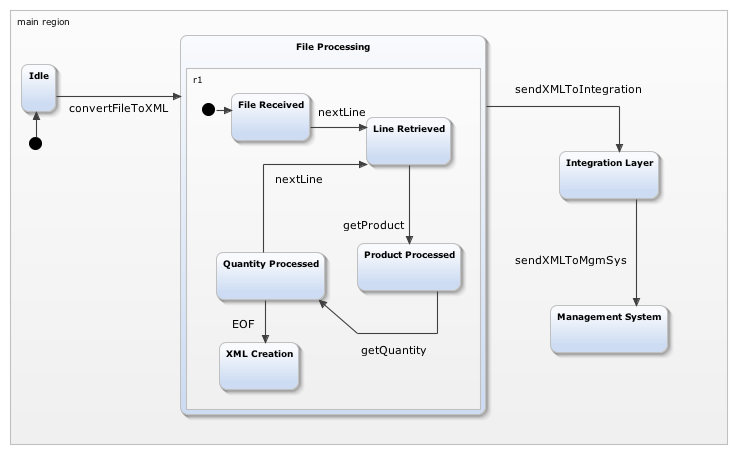
\includegraphics[width=15cm]{figuras/webEDI}
\caption{\label{fig:webEDI} Statechart for order file processing and transference}
\end{figure}

In figure \ref{fig:webEDI}, to contruct the coverage path to \textit{Idle} we do not need to worry about hierarchy, so approach described in the prior section (\ref{testSimpeState}) is enough.

\begin{center}
\begin{tabular}{| l | l|}

\hline

State & Coverage path \\ \hline

Idle & e \\

\hline
\end{tabular}
\end{center}

Notice that once again the empty string $e$ is present due to the unlabeled transition leaving the initial state.

When creating the coverage path for state \textit{File processing}, we notice that it actually is superstate. So, instead, we go deeper in the hierarchy level to obtain the coverage paths of substates \textit{File received, Line retrieved, Product processed, Quantity processed} and \textit{XML creation}. We should add the following paths to set $C$:

\begin{center}
\begin{tabular}{| l | l|}

\hline

State & Coverage path \\ \hline

File received & e convertFileToXML e \\ \hline

Line retrieved & e convertFileToXML e nextLine\\ \hline

Product processed & e convertFileToXML e nextLine getProduct\\ \hline

Quantity processed & e convertFileToXML e nextLine getProduct getQuantity\\ \hline

XML creation & e convertFileToXML e nextLine getProduct getQuantity EOF\\ 

\hline
\end{tabular}
\end{center}

Notice that the coverage path for the superstate \textit{File processing} is removed from $C$, because we are considering its substates. Therefore, the testcases that would be created based on the superstate will be created based on the substates. Besides, the empty string $e$ is added twice in each of these paths. That is beacuse they pass through two initial states with unlabeled transitions: the first one is the general initial states, and the second one is the initial state inside \textit{File processing}.

We still need to cover states \textit{Integration layer} and \textit{Management system}. Observe that to cover these states, we need to pass by \textit{File processing}, a superstate. Therefore, in their coverage path, we need to use a specific notation to guide the later expansion with the substates coverage paths. We will use the notation $\Delta_{File\ processing}$ to indicate that, when creating the test cases, we need to expand the path considering the coverage of \textit{File processing}'s substates. Thus, the coverage paths for \textit{Integration layer} and \textit{Management system} are as follows:

\begin{center}
\begin{tabular}{| l | p{10cm}|}

\hline

State & Coverage path \\ \hline

Integration layer & e convertFileToXML $\Delta_{File\ processing}$ sendXMLToIntegration \\ \hline

Management system & e convertFileToXML $\Delta_{File\ processing}$ sendXMLToIntegration sendXMLToMgmSys\\

\hline
\end{tabular}
\end{center}

At this point, that we have the complete set $C$, we start to in fact create the test cases. As an example, we will examine transitions \textit{getProduct, sendXMLToIntegration} and \textit{sendXMLToMgmSys} more closely.

For \textit{getProduct}, a transition leaving a substate, the process will be the same one presented in the previous section (\ref{testSimpeState}). Hence, we have the following test case:

\begin{itemize}

\item Test case for \textit{\textbf{getProduct}}

Path: \textit{e convertFileToXML e nextLine getProduct}

Expected state: \textit{Product processed}

\end{itemize}

In the case of \textit{sendXMLToIntegration}, a transition that leaves a superstate, we need to use the information regarding the substates to create the test cases. For each substate's coverage path $p$, there will be a test case for \textit{sendXMLToIntegration} making usage of $p$. We should append $sendXMLToIntegration$ to each $p$ in order to obtain the test paths:

\begin{itemize}

\item Test case \#1 for \textit{\textbf{sendXMLToIntegration}}

Path: \textit{e convertFileToXML e sendXMLToIntegration}

Expected state: \textit{Integration layer}

\item Test case \#2 for \textit{\textbf{sendXMLToIntegration}}

Path: \textit{e convertFileToXML e  nextLine sendXMLToIntegration}

Expected state: \textit{Integration layer}


\item Test case \#3 for \textit{\textbf{sendXMLToIntegration}}

Path: \textit{e convertFileToXML e  nextLine  getProduct sendXMLToIntegration}

Expected state: \textit{Integration layer}

\item Test case \#4 for \textit{\textbf{sendXMLToIntegration}}

Path: \textit{e convertFileToXML e  nextLine  getProduct  getQuantity sendXMLToIntegration}

Expected state: \textit{Integration layer}

\item Test case \#5 for \textit{\textbf{sendXMLToIntegration}}

Path: \textit{e convertFileToXML e  nextLine  getProduct  getQuantity EOF sendXMLToIntegration}

Expected state: \textit{Integration layer}

\end{itemize}

As for transition \textit{sendXMLToMgmSys}, the expansion of \textit{Integration layer}'s coverage path is pending. Similarly to what we did for transition \textit{sendXMLToIntegration}, we also need to consider the paths of \textit{File processing}'s substates. Therefore, the test cases for \textit{sendXMLToMgmSys} are:

\begin{itemize}

\item Test case \#1 for \textit{\textbf{sendXMLToMgmSys}}

Path: \textit{e convertFileToXML e sendXMLToIntegration sendXMLToMgmSys}

Expected state: \textit{Integration layer}

\item Test case \#2 for \textit{\textbf{sendXMLToMgmSys}}

Path: \textit{e convertFileToXML e  nextLine sendXMLToIntegration sendXMLToMgmSys sendXMLToMgmSys}

Expected state: \textit{Integration layer}


\item Test case \#3 for \textit{\textbf{sendXMLToMgmSys}}

Path: \textit{e convertFileToXML e  nextLine  getProduct sendXMLToIntegration sendXMLToMgmSys}

Expected state: \textit{Integration layer}

\item Test case \#4 for \textit{\textbf{sendXMLToMgmSys}}

Path: \textit{e convertFileToXML e  nextLine  getProduct  getQuantity sendXMLToIntegration sendXMLToMgmSys}

Expected state: \textit{Integration layer}

\item Test case \#5 for \textit{\textbf{sendXMLToMgmSys}}

Path: \textit{e convertFileToXML e  nextLine  getProduct  getQuantity EOF sendXMLToIntegration sendXMLToMgmSys}

Expected state: \textit{Integration layer}

\end{itemize}

Notice that, in each case, $\Delta_{File\ processing}$ in \textit{Integration layer}'s coverage was replaced by a substate's coverage path.

